\documentclass{article}
\usepackage{multicol}
\usepackage{abstract}
\renewcommand{\abstractnamefont}{\normalfont\bfseries}
\renewcommand{\abstracttextfont}{\normalfont\small\itshape}
\usepackage{titlesec} 
\renewcommand\thesection{\Roman{section}} 
\titleformat{\section}[block]{\large\scshape}{\thesection.}{.75em}{}
\usepackage{graphicx}
\usepackage{wrapfig}

\begin{document}

\title{Blaze Sneakers\\CS 646 Group 2}
\date{\today}

\author{
  King, Tiara\\
  \texttt{@uab.edu}
  \and
  Nettles, AJ\\
  \texttt{arnet@uab.edu}
  \and
  Allison, Leigh\\
  \texttt{leighg@uab.edu}
}
\maketitle

\begin{abstract}
\noindent
    We introduce Blaze Sneakers, a decentralized web application (DApp) for purchasing sneaker images as non-fungible tokens (NFTs).
    The Blaze Sneakers web site allows users to buy images of popular sneakers as tokens (SNKRs) on an Ethereum network.
    Once an account has purchased at least one SNKR, the account owner can view their entire collection on the site.
    NFTs are increasing in popularity, and the proof of ownership provided by blockchain technology enables many uses.
    They could be used to grant access to special web sites or virtual events.
    The number of tokens available is initially limited, but we can add new images/tokens at any time.
\end{abstract}

%\begin{multicols}{2} 

\section{Introduction}
    I sat down to work on this tonight but I was too tired to get anywhere lol.
    Problems with centralization.\\
    Decentralization is better because.\\
    NFT tokens are good.\\
    Sneakers are cool.\\
    Tokens can be used to do cool stuff.


\section{Background}
    Blockchain technology was first introduced with the paper ``Bitcoin: A Peer-to-Peer Electronic Cash System'', 
    published by Satoshi Nakamoto in 2008.
    Satoshi Nakamoto is a fake name, however, so we do not know for certain who invented it.
    Blockchain is a data storage structure that is similar to a linked list, but it is impermeable.
    Each ``block'' is made up of transactions and is built off the previous block, creating a chain that cannot be altered.
    It enables the exchange of virtual currency without requiring a trusted third party.
    It operates in a decentralized fashion, on all computers that are connected to its network, 
    as opposed to on a centralized server.
    \newline
    \indent
    Ethereum is one implementation of blockchain and cryptocurrency.
    Unlike Bitcoin, however, Ethereum was designed for more than simply exchanging currency. 
    It allows the creation of smart contracts, which are Turing complete. 
    It enables developers to create decentralized applications with user interfaces and other decentralized components.
    This new, decentralized focus is known as web3.

\section{Project Description}
    The front-end of the project is a user interface that enables clients to browse and purchase NFTs.
    The back-end is a smart contract, deployed on an Ethereum blockchain.
    When a user visits the home page $( Figure~1 )$, it displays a list of all NFTs currently in the system. 
    Each one is labeled as having been sold, available for purchase, or coming in the future.
    This availability of each token is obtained by calling a function in the contract.
    
\begin{figure}[!h]
    \centering
    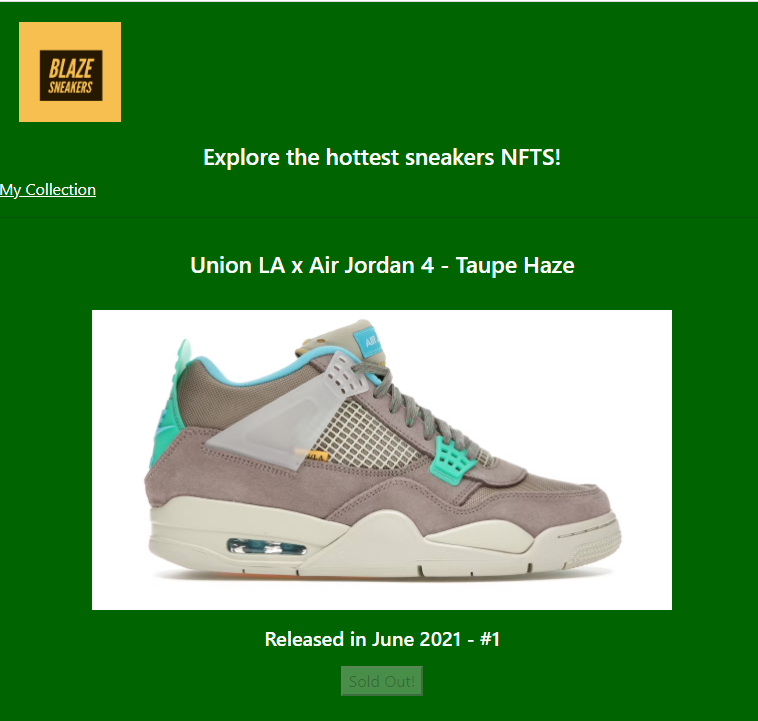
\includegraphics[width=0.4\textwidth]{HomePage.png}
    \caption{Blaze Sneakers Home Page}
\end{figure}
    
    If an NFT is available for purchase, a button is enabled to allow the user to purchase it.
    When the purchase button is clicked, it prompts them with the price and asks if they are certain.
    When a user confirms their intention to purchase a SNKR, another function in the smart contract is called to mint it.
    This function handles the transfer of funds from the user's account to the contract owner's account.
    The user is directed to log in to their Ethereum wallet and choose the account with which to pay $( Figure~2 )$.
    
\begin{figure}[!h]
    \centering
    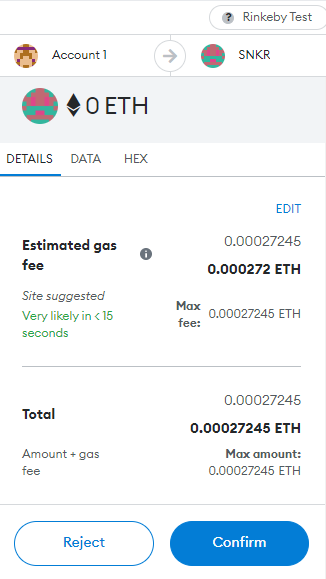
\includegraphics[width=0.25\textwidth]{MetaMaskPurchasing.png}
    \caption{MetaMask Purchasing Example}
\end{figure}

    Once they own at least one SNKR, they can view their collection via the ``My Collection'' link.
    This link goes to a separate page for displaying all SNKRs owned by an account.
    It uses a verify function in the smart contract to determine which tokens are owned by the account.
    \newline
    To add new tokens to the site, we visit a hidden control panel page. 
    This page calls a contract function to confirm whether the user is the contract owner.
    If they are, a button will be displayed for incrementing the number of tokens.
    This button calls another function in the contract to increase the total number of SNKR tokens.
    
    
\section{Design Decisions}
    We chose to write the Ethereum smart contract in the Solidity language and used the Remix online integrated development environment.
    The Solidity code must be compiled into bytecode that runs on the Ethereum network.
    Remix allows us to compile, test, and deploy the contract in one environment.
    We deployed the contract on the Rinkeby testnet. This allows for risk-free testing on a network that does not user real ether.
    \newline
    \indent
    Using the ERC721 standard for NFTs makes the contract interoperable with others who follow the standard.
    OpenZeppelin has a template for ERC721, which makes developing basic NFT functions and following the standard less complex.
    \newline
    \indent
    The NFT image files are stored on the Interplanetary File System (IPFS), as well as in the project's repository.
    IPFS is a decentralized way to store the images, but our implementation requires the user to have IPFS installed and running locally.
    \newline
    \indent
    We chose Visual Studio Code as a development environment for the front end, 
    because it is lightweight and easily customizable.
    We designed the web pages with HTML, using CSS for styling. 
    We used Javascript for the front-end programming logic, including calling the smart contract.
    The web3.js package is provided to handle connecting to the Ethereum network.
    In order to host the site for testing, we used the LiveServer plugin by Ritwick Dey.

\section{Limitations and Future Work}
    IPFS must be installed and running on the client device for the images to be available via IPFS. 
    In the future, we would like to make the contract itself able to access the images.
    This would alleviate the requirement of IPFS on the client.
    Future work: NFT ownership could allow access to private web sites and online events.\\
    Limited and rare editions 

\section{Conclusions}
    Everyone loves sneakers. \\
    Exclusive access to stuff.\\
    Blaze Sneakers is the place to go for sneaker NFTs.

%\end{multicols}
\section{References}
Antonopoulos, Andreas M. and Dr.Gavin Wood. 2019. \underline{Mastering Ethereum}, 
\newline \indent https://github.com/ethereumbook/ethereumbook. (2022).
\newline Nakamoto, Satoshi. 2008. ``Bitcoin: A Peer-to-Peer Electronic Cash System'',
\newline \indent https://uab.instructure.com/courses/1579032/assignments/6671698. (2022)

\end{document}